\documentclass[11pt,a4paper]{book}
\usepackage[utf8]{inputenc}
\usepackage{amsmath}
\usepackage{amsfonts}
\usepackage{amssymb}
\usepackage{graphicx}
\usepackage{url}
\usepackage{lipsum}
\usepackage{marginnote}
\usepackage[disable]{todonotes}

\author{FrontEndART Szoftver Kft.}
\title{User's Guide of the CROSSMINER Advanced Integrated Development Environments Plug-in}

\date{Version 1.15.0.rev0}

\newcommand{\todoi}[1]{\todo[inline]{#1}}

\makeatletter
\renewcommand{\maketitle}{
\vspace*{.1\textheight}
\begin{center}
	
\includegraphics[width=.6\textwidth]{pic/CROSSMINER-logo-large.png}
\end{center}
\begin{center}
	\Huge\@title
\end{center}
\vfill
\begin{center}
	\large\@author\\\@date{} $\bullet$ \today
\end{center}
}
\makeatother

\newcommand{\placeholder}[1]{$\left\langle\text{#1}\right\rangle$}

\newcommand{\SHALL}{\colorbox{red!25}{\textsc{shall}}}
\newcommand{\SHOULD}{\colorbox{orange!25}{\textsc{should}}}
\newcommand{\MAY}{\colorbox{cyan!25}{\textsc{may}}}

\newcommand{\status}[1]{\textbf{Status:} #1}
\newcommand{\todom}{\textcolor{gray}{to do}}
\newcommand{\waitingForServer}{\textcolor{red}{waiting for server side implementation}}
\newcommand{\inprogress}{\textcolor{orange}{partially done}}
\newcommand{\done}{\textcolor{green}{done}}

\newcommand{\unknown}{\colorbox{yellow}{???}}

\usepackage{ifthen}
\newboolean{showreq}
\setboolean{showreq}{false}
\newcommand{\req}[4][\todom]{
\ifthenelse{\boolean{showreq}}{
	\medskip\marginnote{
\includegraphics[width=2.75em]{pic/contract}}\noindent\textbf{\textsf{Requirement #2}} #4  \status{#1}\\\noindent\textit{#3}\bigskip\par
}{}
}

\begin{document}
	
\begin{titlepage}
	\maketitle
\end{titlepage}

\tableofcontents

\chapter{General features}

In this chapter we present several functions which can not be linked to any single feature.
These embodied an overview about the general principles which interwove the whole plug-in.

\section{Installation guide}
Update sites are used to organize and export features so they can be installed into Eclipse applications. A feature is used to package a group of plug-ins together into a single installable and updatable unit. Features have a manifest that provides basic information about the feature and its content. content may include plug-ins, fragments and any other files that are important for the feature. A feature can also include other features. The delivery format for a feature is a JAR, but each included plug-in will be provided as a separate JAR.

\subsection{Create an update site with Eclipse IDE}

First of all, you need to create a feature, from our plug-in. You can create a new feature by creating a New Feature Project. After your feature project is completed, you have to add our plug-in in feature.xml Included Plug-ins tab as Figure~\ref{fig:feature} shows.

\begin{figure}[!h]
	\centering
	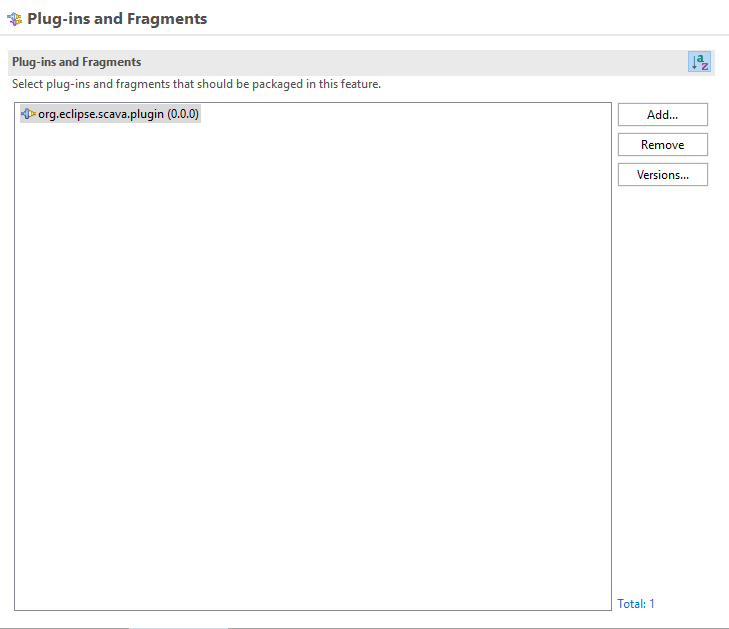
\includegraphics[width=\linewidth]{pic/feature.png}
	\caption{Included plug-ins window}
	\label{fig:feature}
\end{figure}

When your feature is ready, you have to create an update site. You can create a new update site by creating a New Update Site Project. After your update site project is completed, you have to add the feature in site.xml Site Map tab as Figure~\ref{fig:update} shows. After you added the feature to site.xml you can Build an update site.


\begin{figure}[!h]
	\centering
	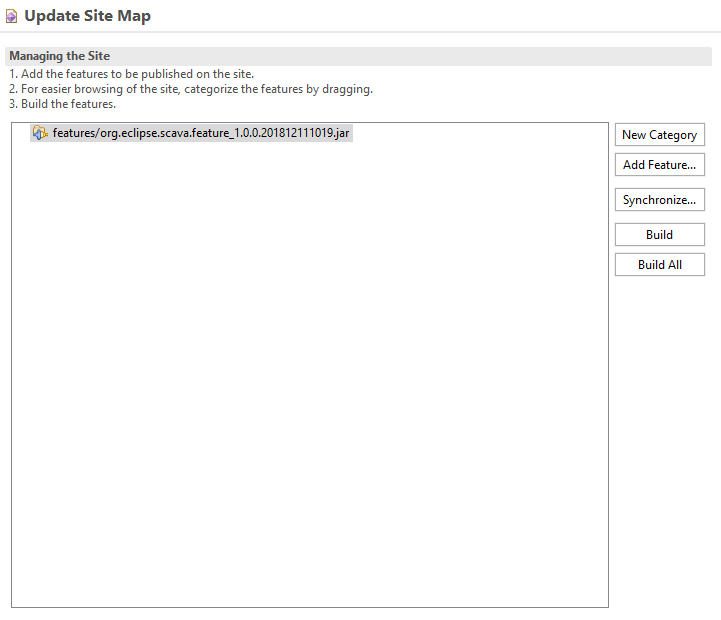
\includegraphics[width=\linewidth]{pic/update_site.png}
	\caption{Site Map window}
	\label{fig:update}
\end{figure}

\subsection{Install plug-in via an update site}

To install plug-in via an update site select the \textit{Install new software} under the Help menu in Eclipse. As you see on Figure~\ref{fig:install_updatesite} the following window you can choose the location of the update site. The location can be a remote or local one. After you select the update site's location it will be shown in the list. You can browse the plug-in's features and disable it if it is not necessary for you. After you are ready, click the \textit{Next} button. On the following screen you have to accept the license agreement if you want to continue the installation. The last screen you see the installation details, on this screen there is a list which contains all of the selected feature for your installation. To finish the installation process click on the \textit{Finish} button.

\begin{figure}[h]
	\centering
	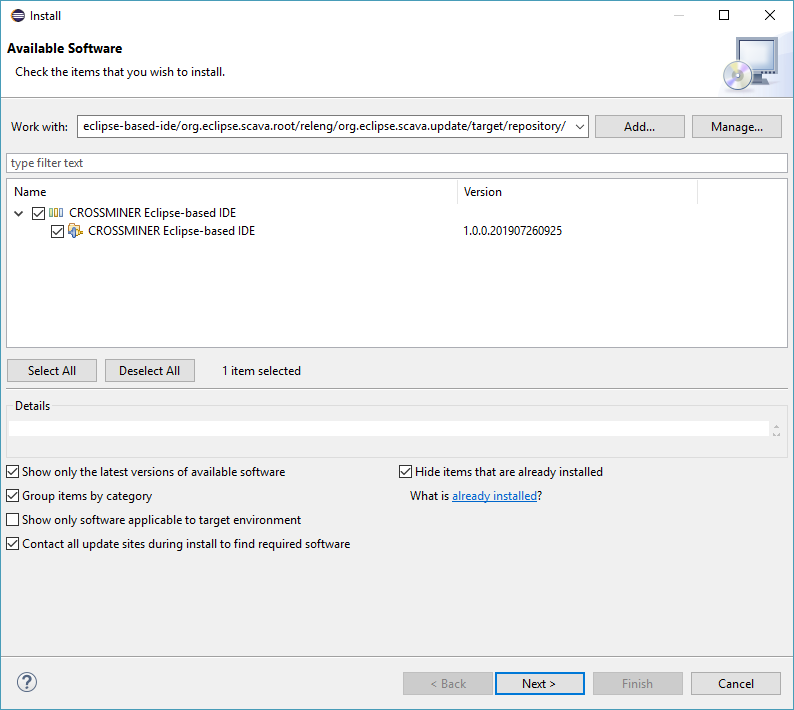
\includegraphics[width=\linewidth]{pic/updatesite.png}
	\caption{Available Software window}
	\label{fig:install_updatesite}
\end{figure}

\req[\done]{U12}{Able to obtain the API results in JSON format}{\SHALL}
\req[\done]{U13}{Able to use the API over REST}{\SHALL}
\req[\done\todo{done up to date}]{U18}{API is utilised by all UIs (dashboard, IDE plugin)}{\SHALL}

\req[\todom]{U154}{Eclipse users can invoke code recommender via an easy shortcut}{\SHALL}
\req[\todom]{U156}{Eclipse IDE proposes a dedicated view or perspective for recommendations}{\SHALL}
\req[\todom]{U158}{Eclipse IDE plugin can be installed via the Marketplace}{\SHALL}
\req[\done]{U159}{Eclipse IDE plugin can be installed via an update site}{\SHALL}

\req[\todom]{U220}{User and admin documentation is embedded into the UI}{\SHALL}
\req[\done]{U225}{Plugin supports the latest supported release of Eclipse}{\SHALL}

\req[\done\todo{up to date}]{D138}{The CROSSMINER REST API shall use UTF-8 encoding for all kind of data sent or received in text mode.}{\SHALL}

\chapter{Acquire Recommendations}

There are several kind of suggestions and recommendation which could be helpful for the developer during their daily tasks. In this chapter we introduce those features which result some kind of recommendation. One of the main properties is the type of entity which are the subject of the suggestion. To simplify any further discussion our tool only permit recommendation with a single subject type. You can find more details in the following sections.

\req[\waitingForServer\todo{Nothing to do directly on IDE side?}]{U1}{Able to extract the development dependencies of a project}{\SHALL}
\req[\waitingForServer\todo{Nothing to do directly on IDE side?}]{U2}{Able to extract the test dependencies of a project}{\SHALL}
\req[\waitingForServer\todo{Nothing to do directly on IDE side?}]{U3}{Able to extract the runtime dependencies of a project}{\SHALL}

\req[\todom]{U157}{Eclipse IDE proposes filtering options for recommendations}{\SHALL}

\req[\waitingForServer\todo{It is a MAY. Howto: e.g. label recommendation as TEST}]{U223}{Provides recommendations to improve test coverage}{\MAY}

\req[\inprogress]{D75}{Recommendation query shall be initiated from the menu, from context menus, and from the toolbar in the IDE. So the user can easily start working with the recommendations.}{\SHALL}
\req[\todom{} \waitingForServer\todo{Some recommendation types needs to be defined in details (with examples).}]{D76}{The IDE shall use a view to list the code recommendations for the examined project. The view shall provide hierarchical grouping of listed items, filtering by meta-properties, and navigation.}{\SHALL}
\req[\waitingForServer\todo{API needs to be defined. According to L'Aquila the server will receive only a string from a prepared set of options.}]{U167}{CROSSMINER IDE provides the ability for the developer to give feedback on the usefulness of the advices in the given situation}{\SHALL}
\req[\waitingForServer\todo{Not IDE! Needed for U167 and D79}]{D105}{The CROSSMINER REST API should provide an interface that allows the user to report if the answer of query previously returned by the API was inappropriate answer for the query. So the knowledge base gets feedback and can be improved.}{\SHOULD}

\section{Library Based Recommendations}

Recommendation which subject are libraries are called \emph{library based recommendations.} This feature helps you to search libraries whiches fit in your development process.

\subsection{Project search}

To search for projects which can be installed into your system, select the Project Search feature under the CROSSMINER menu. After the dialog opened, you can type the desired search expression into the search field. After that, hit enter or click on the Search button. The results are going to show up in a new tab in the middle of the dialog. Every search is going to open a new tab and show up inside that.

On the left part of this tab you can see the results list. Initially only a few of these results are shown in the list, but by clicking on the Show more button at the bottom some more results can be requested. If no more results can be loaded then the button will no longer be available and a short text will inform you about it. By clicking on these items a couple of informations are shown in the right part of the search tab, like a description or the dependencies. You can navigate to the GitHub repository, to the official website of the project or to the related CROSSMINER Web-based Dashboard site. You can initiate a new search for similar projects to the given project by clicking on the similarity method buttons. These are the Compound, Crossim, Dependency, Crossrec, Readme, RepoPalCompound and RepoPalCompoundV2. Or you can select the given project result to be installed by clicking on the Add button in the result's box. The selected projects are shown on the right side of the dialog in a list. By clicking on these items you can view the details of them such like in the previous case. You can deselect these items by clicking on the Remove button. After you chose the wanted projects to be installed click on the Install button on the bottom of the dialog. The search dialog can be seen on the Figure~\ref{fig:projectSearchDialogSearch}.

\begin{figure}[h]
	\centering
	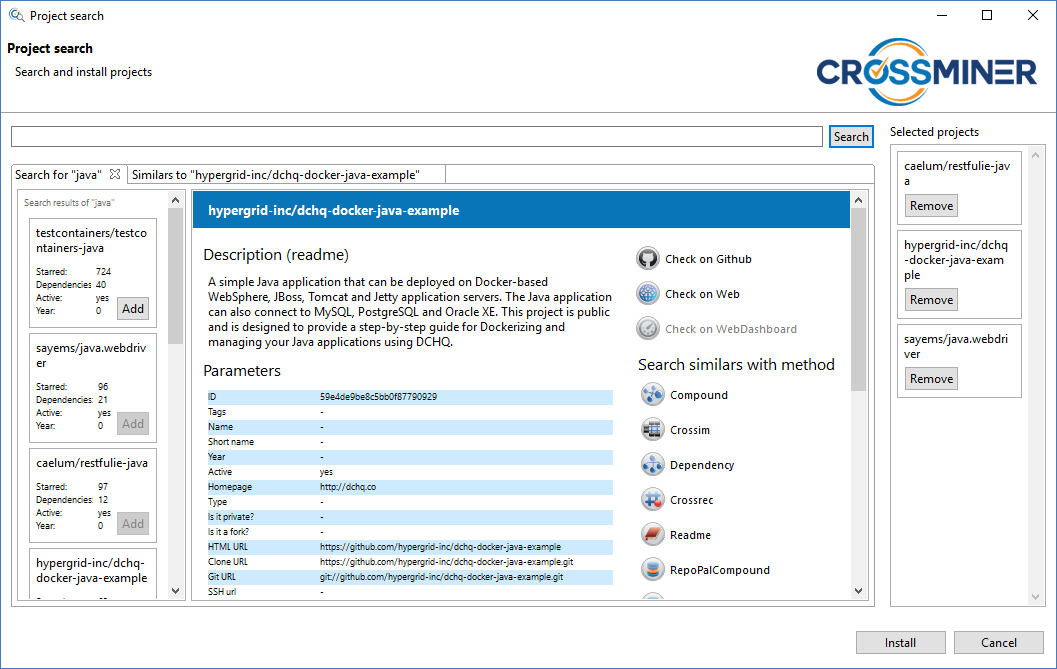
\includegraphics[width=\linewidth]{pic/project-search-search.png}
	\caption{Project search dialog - search}
	\label{fig:projectSearchDialogSearch}
\end{figure}


In the install dialog you can set the base path to the location where you want to install the projects by default. After updating this path all of the projects destination location is going to be updated. You can see this property of the projects on the bottom of the dialog, in the project list. All of the projects can be installed into different locations from the default by giving them a custom destination path. After setting all of the desired install paths, you can choose to install all the projects at once by clicking on the Install all button or you can install them one-by-one manually, by clicking on the Install buttons of the projects. The installation process can be canceled by clicking on the Cancel buttons. The install dialog can be seen on the Figure~\ref{fig:projectSearchDialogInstall}.

\begin{figure}[h]
	\centering
	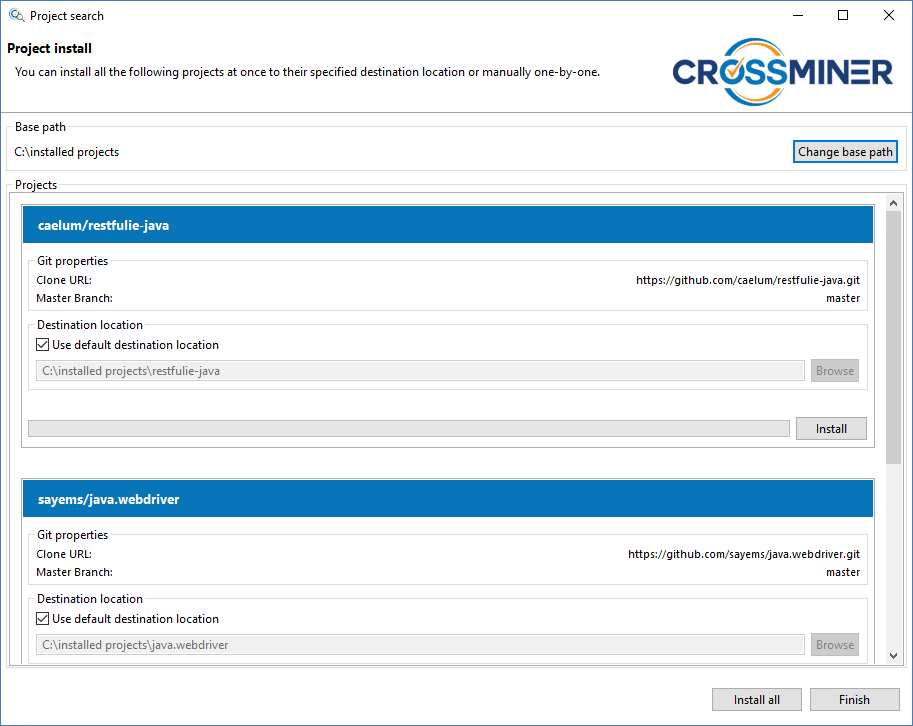
\includegraphics[width=\linewidth]{pic/project-search-install.png}
	\caption{Project search dialog - install}
	\label{fig:projectSearchDialogInstall}
\end{figure}

\subsection{Searching additional libraries}

To search for libraries that can be useful during the development of your project, open the Library search dialog. For this, first you have to select the project in the Package explorer view. This feature works only with Maven projects, that contains their pom.xml file in their root folder. Then navigate in the menu to the CROSSMINER menu and click on the Search libraries option. This will bring up the Library search dialog.

This dialog is split into two parts. On the left side you can see the currently used libraries in your project and on the right side there are the suggested libraries. Both the left and the right side contains their libraries in two separate groups. On the left side, in the upper group there are the libraries that has been selected to be used as the base of the search. The suggested libraries may vary by the different  set of selected libraries. On the bottom there are the libraries that has not been selected yet. On the right side, in the lower group there are the libraries that the CROSSMINER suggested for you to use in your project. The dialog at this state can be seen in the Figure~\ref{fig:librarySearch:results}. These libraries can be selected to be installed, and if they are, then they move to the upper group which contains the libraries that has been selected to be installed. This can be seen on the Figure~\ref{fig:librarySearch:selected}.

\begin{figure}[h]
	\centering
	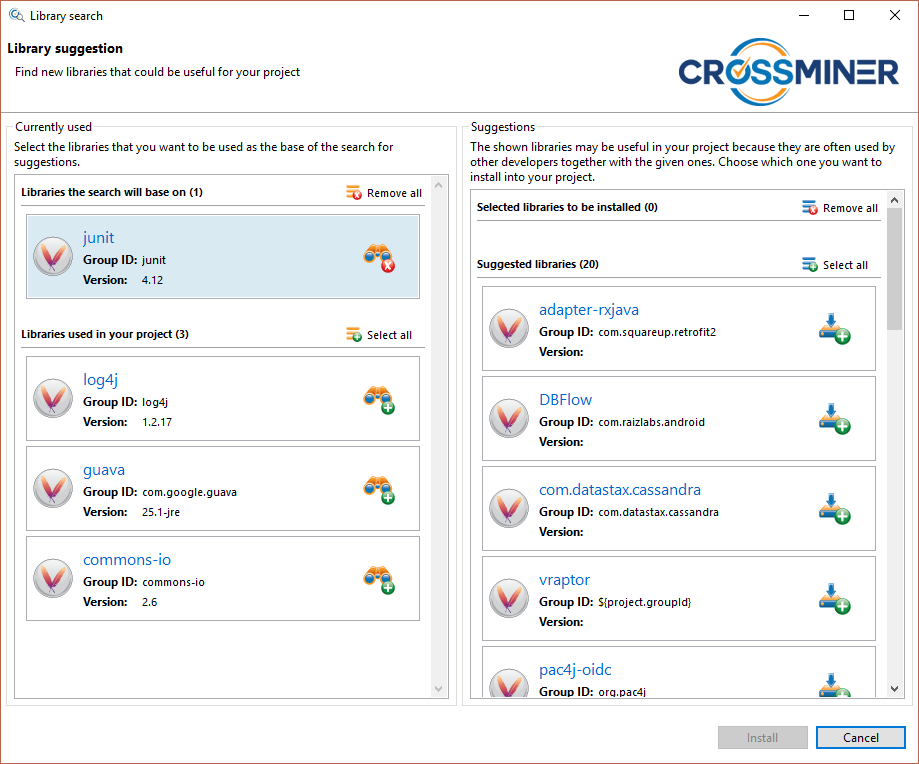
\includegraphics[width=\linewidth]{pic/library-search-results.png}
	\caption{Library search dialog - results}
	\label{fig:librarySearch:results}
\end{figure}

\begin{figure}[h]
\centering
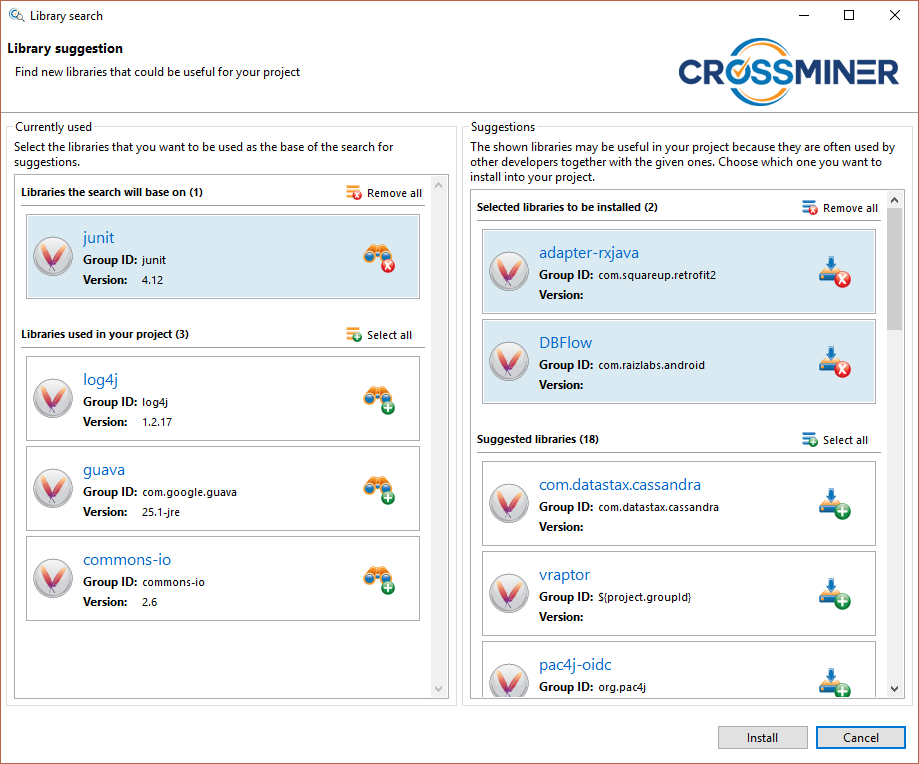
\includegraphics[width=\linewidth]{pic/library-search-selected.png}
\caption{Library search dialog - selected to install}
\label{fig:librarySearch:selected}
\end{figure}

Every time you change the search parameters, so the set of libraries that are used as the base of the search, the suggested libraries will be reloaded. If something goes wrong so the libraries cannot be retrieved from the CROSSMINER server, a Try again button will be shown and by clicking that you can initiate a new request to load them. This is shown in the Figure~\ref{fig:librarySearch:tryagain}.

\begin{figure}[h]
\centering
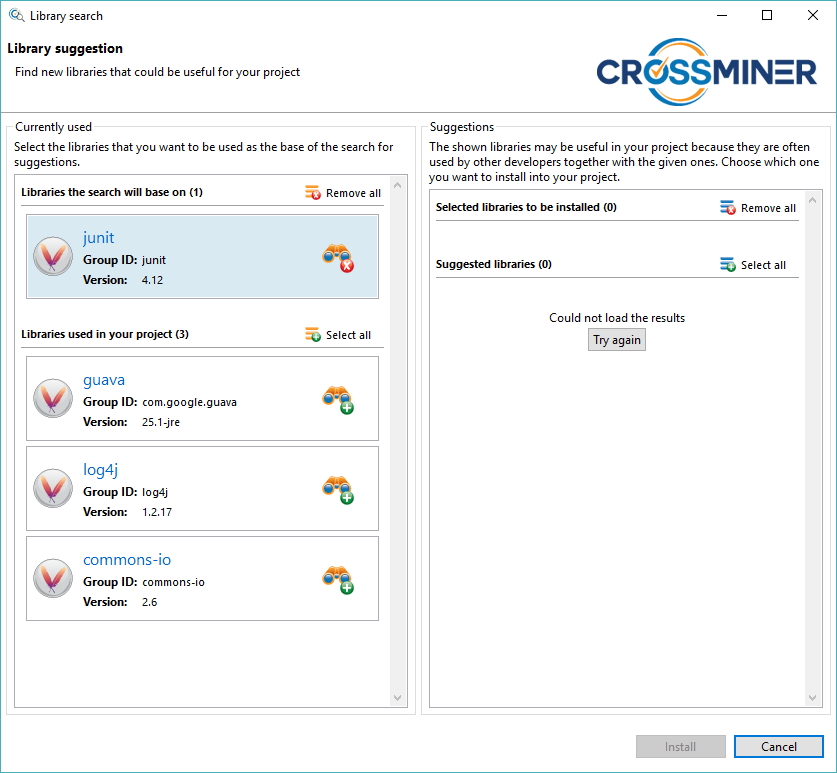
\includegraphics[width=\linewidth]{pic/library-search-try-again.png}
\caption{Library search dialog - try again}
\label{fig:librarySearch:tryagain}
\end{figure}

After selecting the set of libraries that you want to use in your project, by clicking on the install button you can add them to your project. They will show up among the dependencies in the project's pom.xml.

\subsection{Updating libraries}

If any of the libraries that are used in your Maven project can be updated to a newer version the CROSSMINER IDE will notify you by putting the "[new lib version available]" label after the project's name. An example can be seen on the Figure~\ref{fig:libraryVersionChecker}. This check is preformed at the start of the Eclipse IDE.

\begin{figure}[h]
	\centering
	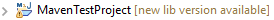
\includegraphics[width=.7\linewidth]{pic/library-version-checker.png}
	\caption{Library version checker}
	\label{fig:libraryVersionChecker}
\end{figure}


To update the libraries that are used in your Maven project use the Library version updater feature. For this, first you have to select your project in the Package explorer view, then in the context menu navigate to the CROSSMINER submenu and click on the "search updates for libraries" option. This will open the Library version updater dialog.

\begin{figure}[h]
	\centering
	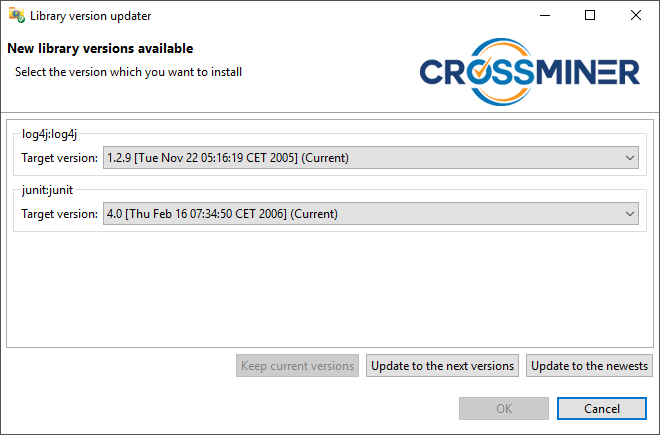
\includegraphics[width=\linewidth]{pic/library-version-updater.png}
	\caption{Library version Updater}
	\label{fig:libraryVersionUpdater}
\end{figure}

As it can be seen on the Figure~\ref{fig:libraryVersionUpdater} the libraries that can be updated to a newer version are listed in the center of the dialog. The different versions can be selected from the dropdown menus and the libraries will be updated to the selected versions.

The listed versions can be filtered by creating rules in the Library update version rules property page that can be accessed by opening the context menu over your project, clicking on the Properties option and navigating under the CROSSMINER pages.

Any number of rules can be added, removed or edited in this page. To create a new rule click on the Add new rule button. A box will appear in the center of the page with three text fields. These fields are the Group ID, the Artifact ID and the Version. Each field can be filled with regular expressions and they are interpreted just the same way as in Java. If a text field has been leaved empty it will be interpreted as to match with every value.

The rules can be removed by clicking on the "Delete rule" button in the rule's box.

This property page and an example rule can be seen on the Figure~\ref{fig:libraryVersionRules}. With this one rule we restrict the library version search to care only about the libraries with a group ID that matches with 'junit', an artifact ID, that matches with 'junit' and a version with a '4.' prefix.

\begin{figure}[h]
	\centering
	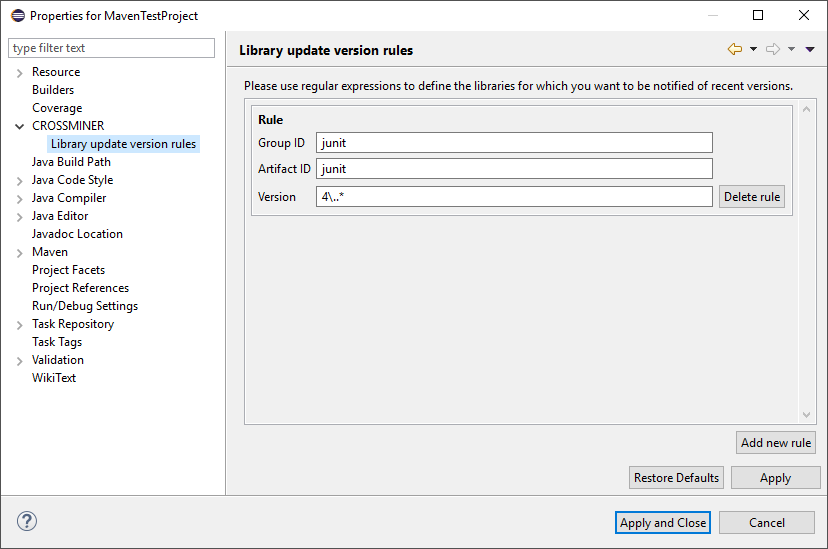
\includegraphics[width=\linewidth]{pic/library-version-rules.png}
	\caption{Library version rules}
	\label{fig:libraryVersionRules}
\end{figure}

The interpretation of the rules is the following:
if there are no rules at all, then no filtering will be applied.
After adding at least one rule, then the library versions will be tested against every rule until at least one of them is matching. If none of the rules matched a library version, then that one will not be seen among the available library versions. A filtered list of library versions with the previous rules can be seen on the Figure~\ref{fig:libraryVersionUpdater:filtered}.

\begin{figure}[h]
	\centering
	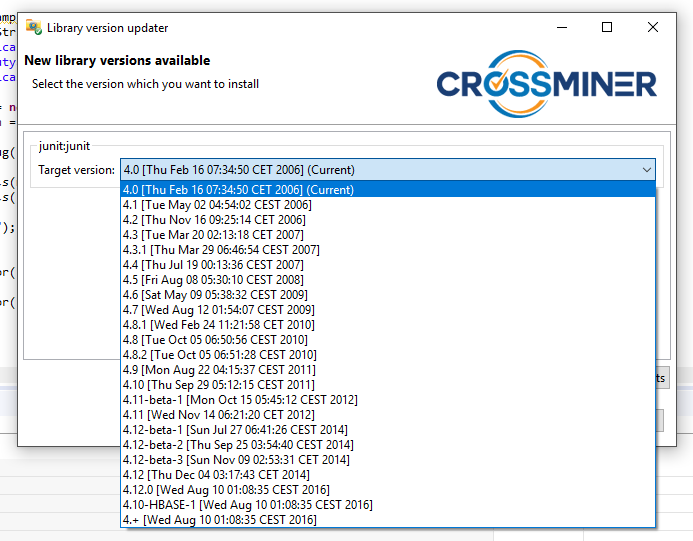
\includegraphics[width=\linewidth]{pic/library-version-updater-filtered.png}
	\caption{Library version Updater - filtered}
	\label{fig:libraryVersionUpdater:filtered}
\end{figure}

In the Library version updater dialog there are three buttons on the bottom, which can be used to quickly select the wanted versions. These buttons provide the functionality to select the currently used, the next available or the latest versions with a click.

After selecting the versions to be installed and accepting the confirmation dialogs, the selected versions of the libraries are going to be installed to your project.

If the upgrade from an older version of a library to a newer one involves some API braking changes, then the CROSSMINER Eclipse-based IDE will try to find the places of usage of the old API in the project and mark them as they are suspicious to be broken after the installation. The markers can be seen on the Figure~\ref{fig:libraryVersionUpdater:apiMigration}.

Hovering you cursor over these markers the quick fix menu can be opened and the following options can be selected: you can choose the Fix option which will try to fix the broken part of the API usage near the marked code chunk. The Fix all and Fix all for API migration from old library to new library options will try to do the same but for every similar case in the whole project and to every similar case in the project, but only for those, that are related to the given API migration, respectively. The Ignore options may be interpreted in the same way, but not changing any part of the code, they are just removing the markers from the suspicious code chunks.

\begin{figure}[h]
\centering
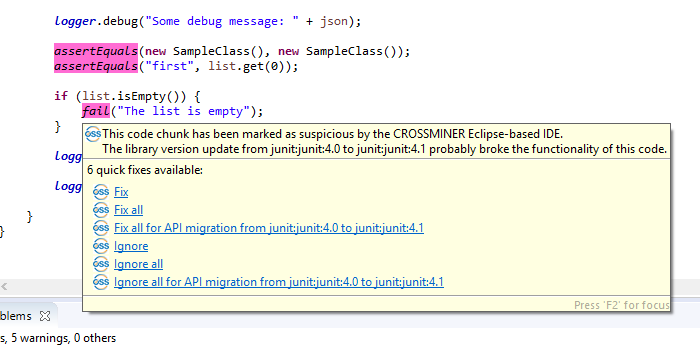
\includegraphics[width=\linewidth]{pic/library-version-updater-api-migration.png}
\caption{Library version Updater - API Migration}
\label{fig:libraryVersionUpdater:apiMigration}
\end{figure}


\req[N/A\todo{WEB Dashboard functionality}]{U4}{Able to warn about superfluous dependencies}{\SHOULD}
\req[N/A\todo{WEB Dashboard functionality}]{U5}{Able to warn about overly precise dependencies}{\SHOULD}

\req[\done]{U81}{Able to identify and list the third-party components used in a project.}{\SHALL}
\todoi{U81: If we can support all case studies, then the current, client-side maven-based identification is enough.}

\req[\inprogress]{D78}{The IDE shall provide an interface to the user, where libraries that match some recommendations are listed with their selected set of details in filterable and sortable form. So the developer can easily compare the libraries and choose those best fit to their expectations.}{\SHALL}
\req[\waitingForServer]{D79}{The IDE should provide the ability to the user to mark a library proposed for a query as ``not appropriate''. This information can help in the improvement of the knowledge base.}{\SHOULD}
\req[\done]{D80}{The IDE shall provide an interface where known information from a single library is shown. This interface can help the user to check details of the library, and reach out for more information through links (e.g. to project home page).}{\SHALL}
\req[\waitingForServer\todo{Not IDE! Needed for D78}]{D100}{The CROSSMINER REST API shall provide an interface that accepts a name and version description and returns the library that is described by them.}{\SHALL}
\req[\done\todo{Not IDE! Needed for D78}]{D101}{The CROSSMINER REST API shall provide an interface that accepts a library and returns detailed information about it (including description, metric values, URLs).}{\SHALL}

\req[\waitingForServer\todo{Source code recommendation on the IDE side, ready.}]{U172}{CROSSMINER IDE provides developers code templates and example of codes related to the usage of the API of a specific project}{\SHALL}
\req[\todom{} \waitingForServer\todo{On the IDE side, it is a free text search (with some pre-defined constraints, if needed.)}]{D77}{The IDE shall provide an interface, where recommendations against a new (to-be-used-in-the-project) library can be given. So the user can describe features and functionalities they wants to perform using an external library. The user can also give some constraints, e.g. minimal age or users of the library.}{\SHALL}

\req[\waitingForServer]{U172}{CROSSMINER IDE provides developers code templates and example of codes related to the usage of the API of a specific project}{\SHALL}
\todoi{U172: A new sub-type of code recommendations is needed to handle code templates.
The KB will send only the changes of the API, which have to be applied on the client side.
The details of the communication must be defined.}

\req[\todom{} \waitingForServer\todo{On the IDE side, it is a free text search (with some pre-defined constraints, if needed). Free text search is okay as far as it satisfies all the use cases.}]{D77}{The IDE shall provide an interface, where recommendations against a new (to-be-used-in-the-project) library can be given. So the user can describe features and functionalities they wants to perform using an external library. The user can also give some constraints, e.g. minimal age or users of the library.}{\SHALL}

\req[\inprogress{} \waitingForServer\todo{Not IDE! Needed for D77.}]{D99}{The CROSSMINER REST API shall provide an interface that accepts a description and some filtering constraints and returns a list of libraries that match with the description and fulfil the constraints.}{\SHALL}

\req[\waitingForServer\todo{Not IDE! Needed for U174}]{D102}{The CROSSMINER REST API shall provide an interface that accepts a library, a description and some filtering constraints and returns a list of libraries that match with the description, fulfill the constraints, and can be used as a replacement to the given library.}{\SHALL}

\req[\waitingForServer\todo{Not IDE! Needed for D81}]{U174}{CROSSMINER IDE provides suggested alternatives to the usage of third-party jar which offer the same range of services as a jar used in current project}{\SHOULD}
\req[\todom{} \waitingForServer]{D81}{The IDE shall provide an interface to the user, where recommendations for replacing a library used in the current project with some alternative libraries can be given. The user can select the library currently used in the project to be replaced and can give further recommendations against the alternatives.}{\SHALL}

\subsection{Handling Changed and Deprecated APIs}

Third party libraries are prone to change and evolution.
To help the developers adapt their project to these changes we defined an other sub-category of recommendations, namely when their goal is to provide information about modified or deprecated interfaces.

\req[\waitingForServer\todo{Not IDE! Needed for U160-162, U164, U168, U169}]{U70}{Able to identify the list of changed third-party API methods from the source code of the third-party API}{\SHALL}
\req[\waitingForServer\todo{Not IDE! Needed for U160-162, U164, U168, U169}]{U71}{Able to identify the list of deprecated third-party API methods from the source code of the third-party API}{\SHALL}
\req[\waitingForServer\todo{Not IDE! Needed for U160-162, U164, U168, U169, U173, U175}]{U72}{Able to determine migration pattern from two (or more) code snippets when one of them uses the old third-party API and the other uses the new third-party API}{\SHALL}

\req[\waitingForServer\todo{Not IDE! Nedded for U160-162, U164, U168, D83-84}]{U80}{Able to detect from the configuration settings if a new version of a used third-party library is available}{\SHALL}
\req[\waitingForServer\todo{Not IDE! Nedded for U160-162, U164, U168, D82-84}]{U130}{Able to identify if the developer is not using the most recent version of a library and provide notification}{\SHALL}

\req[\todom{} \waitingForServer]{U160}{CROSSMINER IDE notifies if a new version of a third-party API used by the project on which the developer is working is available}{\SHALL}
\req[\todom{} \waitingForServer]{U161}{CROSSMINER IDE notifies if a new version of a third-party API used by the project on which the developer is working breaks backward compatibility}{\SHALL}
\req[\todom{} \waitingForServer]{U162}{CROSSMINER IDE is able to offer the use of the newest version of a third-party API utilised in the project}{\MAY}
\req[\inprogress{} \waitingForServer]{U163}{CROSSMINER IDE is able to identify and navigate to those places that became suspicious for changing behaviour after the third-party API version used in the project has changed}{\SHALL}
\req[\inprogress{} \waitingForServer]{U164}{CROSSMINER IDE is able to mark the usage of deprecated third-party APIs in the source code the developer is working on.}{\SHALL}
\req[\todom{} \waitingForServer]{U168}{CROSSMINER IDE is able to notify the developer about third-party API changes that are in design or development phase}{\MAY}
\req[\todom{} \waitingForServer\todo{Summary on IDE side}]{U169}{CROSSMINER IDE is able to provide an overview of the impact of a third-party API change on the project the developer is working on}{\MAY}
\req[\inprogress{} \waitingForServer\todo{Howto: simply insert the received snippet}]{U173}{CROSSMINER IDE assists developers to migrate the current version of a third-party jar to the new version by providing a list of required changes, advices and code templates}{\SHALL}
\req[\inprogress{} \waitingForServer\todo{Howto: simply insert the received snippet}]{U175}{CROSSMINER IDE assists developers to address a deprecated API by proposing an alternative for obtaining the same behaviours of the code}{\SHOULD}

\req[\todom{} \waitingForServer]{D82}{The IDE shall provide the user the ability to initiate library version check. So the user is notified if some libraries used in their project have new versions.}{\SHALL}
\req[\todom{} \waitingForServer]{D83}{The IDE shall perform library version checks on the libraries used in the current project. The check is performed on project load, and only marks the upgradeable libraries.}{\SHALL}
\req[\todom{} \waitingForServer]{D84}{The IDE shall be able to show if a library used in the current project has a new version that satisfies some pre-determined criteria set globally for library upgrades by the user. So the user can see the relevant results of the library upgrade search.}{\SHALL}
\req[\inprogress\todo{ready, up to date}]{D85}{The IDE shall provide an interface where the details of an available library upgrade can be shown. These may include the new version number, release date, number of users, number of bugs, estimated impact of the upgrade, etc.}{\SHALL}
\req[\inprogress{}\todo{ready, up to date}]{D86}{The IDE should provide the ability to initiate a library upgrade that marks all those places in the source code that needs rework due to the change of the library version.}{\SHOULD}
\req[\inprogress{}\todo{ready, up to date}]{D88}{The IDE may perform the steps of a library upgrade autonomously (if the user requested the upgrade).}{\MAY}
\req[\inprogress{} \waitingForServer\todo{Not IDE!}]{D103}{The CROSSMINER REST API shall provide an interface that accepts a library and filters, and returns a list of versions available for that library and match the filters.}{\SHALL}
\req[\waitingForServer\todo{Not IDE! Needed for D86, D88}]{D104}{The CROSSMINER REST API shall provide an interface that accepts a library and two versions, and returns the differences between these library versions. Differences include removed, deprecated, changed, new API elements, and API elements with changed behaviour.}{\SHALL}

\section{Source Code Based Recommendations}

In this section we elaborate features related to those recommendation which subject entities are present in the source code of the project under development. They usually retrieve some code chunk, which could be annotated to ease further understanding.

\subsection{Code recommendation}

Code recommendations are used to retrieve code snippets which may be useful for you by showing an example implementation if a specific library or just presenting a pattern that can be followed. These snippets can be requested by selecting a chunk of code in an open Java source code editor and by clicking on the Request code recommendation option in the context menu's CROSSMINER submenu or by using the Ctrl+Shift+X C key combination. After the Code recommendation view has shown up the suggested patterns for this file will be displayed on the left side in a hierarchical representation. The results are grouped by the file, they are relevant to and by the query, which represents the request for the recommendations at a given time using a given part of the file. This can be seen in the Figure~\ref{fig:codeRecommendation:results}.

\begin{figure}[h]
	\centering
	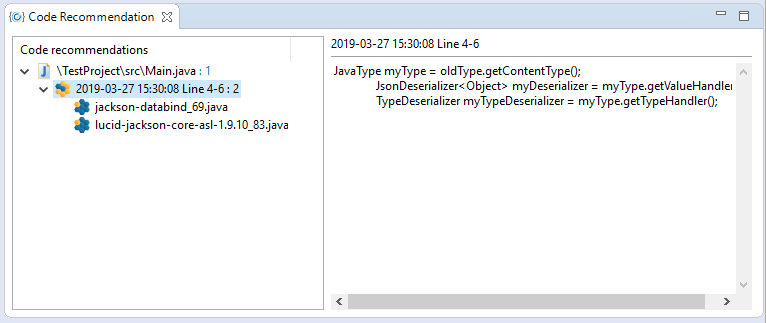
\includegraphics[width=\linewidth]{pic/code-recommendation-results.png}
	\caption{Code recommendation view - suggested patterns }
	\label{fig:codeRecommendation:results}
\end{figure}

By selecting a pattern in the hierarchical tree view the recommended snippet will be shown in the preview view on the right side of the Code recommendation view. Here you can examine the given code, copy a part of it or by using the Insert snippet at cursor button you can paste it into the active editor at the cursor's position or replace the selected code chunk with it. This functionality is available only when there is an active editor opened. The preview view can be seen on the Figure~\ref{fig:codeRecommendation:preview}.

\begin{figure}[h]
	\centering
	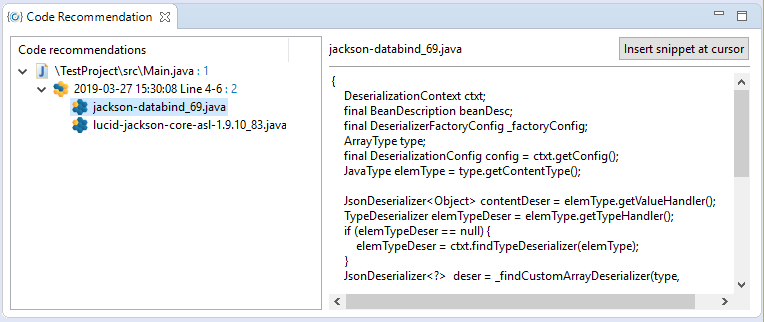
\includegraphics[width=\linewidth]{pic/code-recommendation-preview.png}
	\caption{Code recommendation view - preview snippet }
	\label{fig:codeRecommendation:preview}
\end{figure}

You can also remove the recommended code snippets from the results by opening the context menu over them and choosing the right option for you. Basically there are 4 options that you can go with. If you select a file you have the option to drop all the recommendation that are related to that file. If you select the recommendation query, you can drop all results for that request. If you select the code recommendations you can drop the items one-by-one. Or in all cases there is an option to drop all the recommendations, and this will clear the results view.

By double clicking on a file you can easily navigate to it and request the Eclipse to open it.

\req[\inprogress\todo{Not IDE! Needed for U170-171...}]{U73}{Able to identify the part of the API that the developer is currently using to provide code snippets in relation with current development activity}{\SHALL}
\req[\inprogress{} \waitingForServer\todo{no data for ``as suspicious''}]{U170}{CROSSMINER IDE provides the ability for the developer to ask recommendations for a code chunk previously marked by the CROSSMINER IDE as suspicious}{\SHOULD}
\req[\done]{U171}{CROSSMINER IDE provides the ability for the developer to ask recommendation for an arbitrary code chunk or code element}{\SHOULD}

\req[\inprogress]{D92}{The IDE should provide the ability to the user to select a code snippet or a file and ask for code recommendations for it. So the user can check whether there is a better practice to solve her problem.}{\SHOULD}
\todoi{D92: Code recommendations for arbitrary code is enough.
The CROSSMINER API should provide a point where context information (the whole project?) can also be uploaded (Davide said that it already exists).
The content and form of it must be discussed.}

\req[\inprogress]{D93}{The IDE should be able to show recommendations assigned with code elements. So the user can see what the knowledge base suggested for a code snippet.}{\SHOULD}
\todoi{D93: Code recommendations for arbitrary code can be enough, but the CROSSMINER API can also provide a point for code element recommendations.
The CROSSMINER API should provide a point where context information (the whole project?) can also be uploaded (Davide said that it already exists).
The content and form of it must be discussed.}

\req[\waitingForServer\todo{Not IDE! Needed for U170-171, D91-94}]{D107}{The CROSSMINER REST API may provide an interface that accepts code snippets and library context, and returns recommendations on how to improve that part of the code.}{\MAY}

\req[\done\todo{done, up to date}]{D91}{The IDE may insert a recommendation in the code if the user accepts it and requested it on a code position.}{\MAY}
\req[\inprogress{} \waitingForServer\todo{``IDE replaces ...'' will probably not be implemented, unless the server gives proper recommendations}]{D94}{The IDE may be able to process recommendations and perform code migration autonomously. So the user can point to a recommendation and the IDE replaces the old code to the new one.}{\MAY}
\req[\waitingForServer\todo{Not IDE! Needed for U170-171, D91-94}]{D106}{The CROSSMINER REST API may provide an interface that accepts a list of libraries and a description and returns recommendations about how to implement the described functionality using the given libraries.}{\MAY}

\section{Text Based Recommendations}

Finally there are tons of documentation and discussion available for various topics, which could be useful for the developers. Those recommendations which yield some natural language documents (or reference to them) are called \emph{text based recommendations.}

\subsection{API documentation and Q\&A posts}

This feature is used to show the user some documentation or forum posts where she may find some useful information about the API calls that she is using in her code. To initiate a request for these recommendations you have to select a code chunk in an active editor and click on the Request API documentation and Q\&A posts options the context menu's CROSSMINER submenu. After this, the results are shown in a particular view, where you can examine these results, copy the link for them or by clicking on the title they can be opened in an external browser. This view can be seen on the Figure~\ref{fig:apiDocumentation:results}.

\begin{figure}[h]
	\centering
	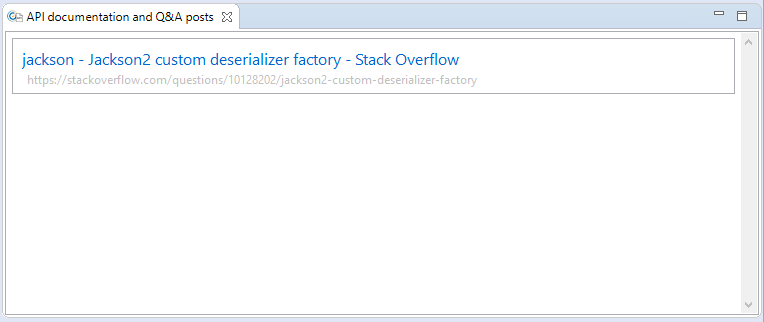
\includegraphics[width=\linewidth]{pic/api-documentation-results.png}
	\caption{API documentation and Q\&A posts view - results}
	\label{fig:apiDocumentation:results}
\end{figure}


\subsection{API Usage}

Developers could use these recommendation to get more information about the features and their usage of a 3rd part API, for example official pages, documentations, and samples.

\req[\todom{} \todo{It is a MAY. Davide said that the API is prepared for sending context-data}\waitingForServer]{D89}{The IDE may provide an interface where description of a feature to be implemented and libraries that should be used to implement it can be given. So the user can ask for recommendations how to implement features using specific libraries.}{\MAY}
\req[\todom{} \todo{It is a MAY. Davide said that the API is prepared for sending context-data}\waitingForServer]{D90}{The IDE may provide an interface to show recommendations on how to implement a feature using some specific libraries.}{\MAY}

\subsection{Handling API changes}

There several forum threads and change reports, which could ease the migration between different versions of the same library.

\req[\todom{} \waitingForServer]{U165}{CROSSMINER IDE offers a list of community discussion forums concerning the use of a changed third-party API element}{\SHOULD}
\req[\todom{} \waitingForServer]{U166}{CROSSMINER IDE offers code examples for deprecated third-party API usage points}{\SHOULD}
\req[\todom{} \waitingForServer]{D87}{The IDE shall provide an interface that explains the steps of how to upgrade a library used in the project to a new version.}{\SHALL}

\chapter{User Activity Monitoring}

The main components of this scenario is the recording of developer interactions (events), computing process related metrics and sending them to the CROSSMINER server for further processing. The collected events is stored in a local database. Please note that none of the stored event contains information about the user, so there is no way to identify someone from these data, also all of the events are stored in a local database and only the metrics are sent to the CROSSMINER Server.

\section{Database settings}

The events are stored in a local database. This database default locate at Workspace location. To change this location you have to open Database preference page under the CROSSMINER tab as figure~\ref{fig:database:settings}. After you change the location it needs an Eclipse restart.

In this page you can also delete your local database. After deletion it also need an Eclipse restart.

\begin{figure}[h]
	\centering
	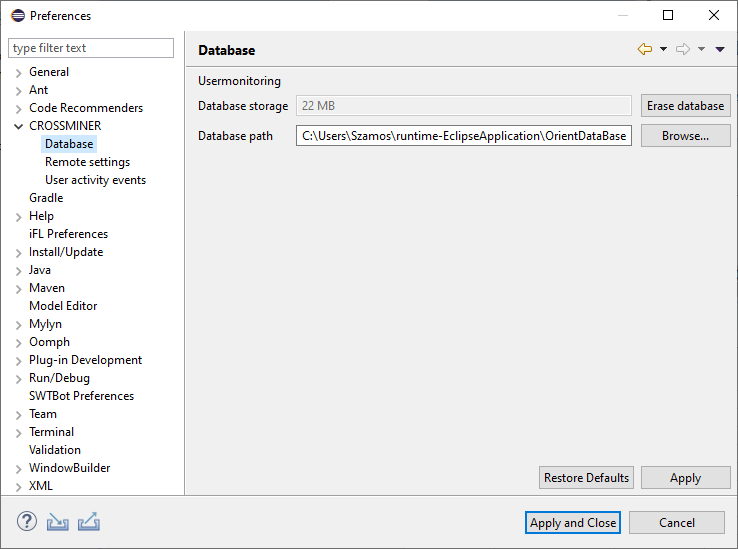
\includegraphics[width=\linewidth]{pic/database_settings.png}
	\caption{Preference page for database settings}
	\label{fig:database:settings}
\end{figure}

\section{User Activity Monitoring Settings}

In the User activity events tab you can customize which events are you want to collect or which metric are you want to compute. As figure~\ref{fig:useractivity:settings} shows. If you disable an event which is required to calculate a metric, hence that metric won't be computed.

\begin{figure}[h]
	\centering
	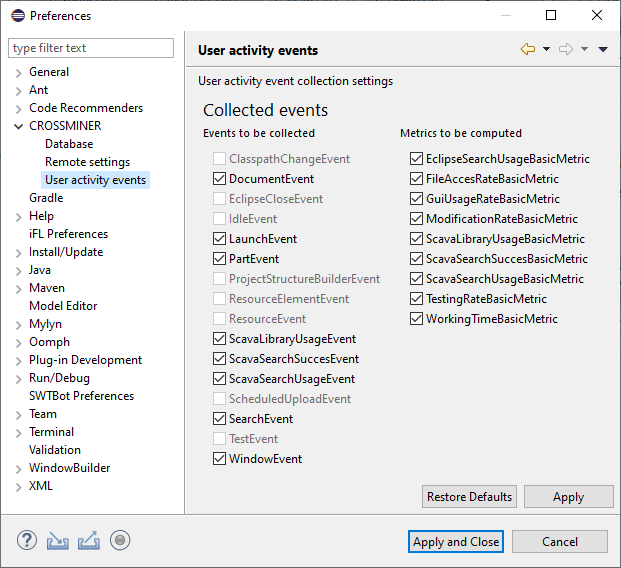
\includegraphics[width=\linewidth]{pic/usermonitor_settings.png}
	\caption{Events and metrics settings}
	\label{fig:useractivity:settings}
\end{figure}


\section{List of Collected Events}

\begin{description}
\item[Document event] Our plug-in using it to detect all keypresses in the editor and store which file is affected. For example during the implementation of a new method for an existing class.

\item[Part event] It stores information about life cycle of given parts (part activating, part deactivating, part closing etc). For example when you work on a existing class and select something in the Package Explorer.

\item[Window event] It stores information about window life cycle the same way as the Part event handles information about parts. For example when you open an another program.

\item[Eclipse close event] Eclipse closes are stored in this even type.

\item[Launch event] It stores information about code building and launching.

\item[Resource element event] It stores information about the file saving and deletion.

\item[Class path event] It stores information about class path changing (add entry to class path or removed entry from class path). For example when you add a library to your clashpath.

\item[CROSSMINER event] These events are invoked by using plug-in. It needs to be calculated for those metrics which measure the plug-in usage. For example when you use CROSSMINER Library Search function.
\end{description}

\section{List of Recorded Metrics}\todoi{Add currently calculated metrics with precisse def (user computable). clearify it with any number of formula if needed}



\req[\todom\todo{Not specific to IDE}]{U176}{There is a strict and public strategy regarding privacy and data}{\SHALL}
\req[\todom{} \waitingForServer\todo{Not specific to IDE}]{U177}{Users cannot be identified from monitoring data}{\SHALL}
\req[\inprogress]{U178}{Monitoring is able to identify testing activities}{\SHOULD}
\req[\done]{U179}{Monitoring is able to identify development activities}{\SHOULD}
\req[\unknown\todo{This needs to be clarified}]{U180}{Monitoring is able to identify errors in IDE}{\SHOULD}
\req[\inprogress]{U181}{Monitoring records the time the developer works on a given file/code element/line}{\SHOULD}

\req[\inprogress]{U218}{All metrics are documented, motivated, possibly with references}{\SHALL}

\req[\todom\todo{Details needs to be defined. Search expressions come only from searches in the plug-in.}]{D96}{The IDE shall recognize, compute, and extract the following user activities, metrics, or information: frequent search expression.}{\SHALL}
\req[\inprogress\todo{Search patterns come only from searches in the plug-in.}]{D97}{The IDE should recognize, compute, and extract the following user activities, metrics, or information: project or file open, manipulation, close, program execution, test execution, user search patterns, working time on a file.}{\SHOULD}
\req[\waitingForServer\todo{Not IDE! Needed for U176-181, D96-98}]{D108}{The CROSSMINER REST API shall provide an interface that accepts developer activity data. So the CROSSMINER can build this information in the knowledge base.}{\SHALL}

\section{Retrieving Process Metrics via \textsc{crossminer} Web-based Dashboard}

You are able to inspect any computed process metrics for your project by using the relevant features of .

\section{Plug-in Side Debugging Features}

In the case of unexpected errors during the user activity monitoring, you are able to check the value of the process metrics and some relevant meta-data about the underlying database on the client side. To do this please activate some of the plug-in side debugging features. Please note that these are only available in the debug version of the plug-in. 

\section{Server Side Debugging Features}

There are ways to access the raw data, stored at the server side. To do this you have to execute the following REST API calls. You could use your preferred REST client, but for illustration purposes we will use Postman\footnote{\url{https://www.getpostman.com/}}

\req[\todom]{D98}{The IDE shall be able to send developer activity data (as controlled by the user settings) to the CROSSMINER server.}{\SHALL}

\chapter{Settings and Customization}


\req[\todom\todo{Not IDE!}]{U155}{Eclipse users can easily deactivate the analysis}{\SHALL}

All the plug-in related settings can be found in the plug-in's preference page. To open this page select the Preferences item under the Window menu in Eclipse menu.



\section{Integration Related Settings}

To properly use the plug-in, you have to set some of the settings which is required for integration. As Figure~\ref{fig:preferences_remote} shows you have to enter the Knowledge Base server address, a port and the Web Dashboard's base path.

\begin{figure}[h]
	\centering
	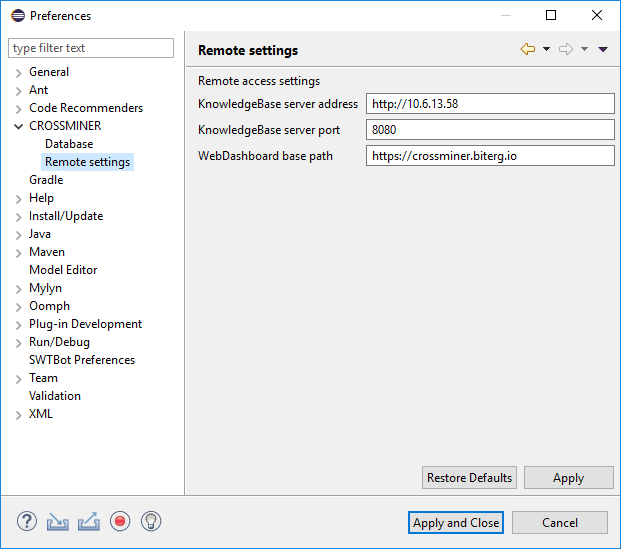
\includegraphics[width=\linewidth]{pic/preferences_remote.png}
	\caption{Plug-in remote settings}
	\label{fig:preferences_remote}
\end{figure}

\req[\inprogress]{D74}{The IDE shall provide a settings interface to the user, where the different properties of the CROSSMINER IDE plugin (like server address and port, global settings for recommendation queries, etc.) can be checked and changed. So the user can configure the plugin.}{\SHALL}

\section{Process Metric Related Settings}

\req[\todom]{U182}{Monitoring of developer activity can be disabled by the developer}{\SHALL}
\req[\todom]{U183}{Types of data collected from monitoring are transparent to the developer}{\SHALL}
\req[\todom]{D95}{The IDE shall provide full control over the collected and transferred user activity monitoring data. So the user can allow or deny the collection and/or anonymised transfer of the activity data collected from their session.}{\SHALL}

\end{document}
